\documentclass[twocolumn]{aastex631}
\makeatletter
\def\ps@plain{%
  \let\@mkboth\@gobbletwo
  \def\@oddhead{}%
  \def\@evenhead{}%
  \def\@oddfoot{\hfil\thepage\hfil}%
  \def\@evenfoot{\hfil\thepage\hfil}%
}
\let\ps@headings\ps@plain
\let\ps@myheadings\ps@plain
\let\ps@article\ps@plain
\let\ps@aas@headings\ps@plain
\def\@journalinfo{}
\def\@slugcomment{}
\def\frontmatter@title@above{}
\makeatother
\pagestyle{plain}
\usepackage{amsmath}
\usepackage{graphicx}
\usepackage{booktabs}
\usepackage{array}
\usepackage{microtype}
\newcommand{\kms}{km\,s$^{-1}$}
\renewcommand{\bibfont}{\tiny}

\begin{document}
\pagestyle{plain}
\sloppy
\hbadness=10000
\hyphenpenalty=10000
\exhyphenpenalty=10000

\title{Empirical Response Exponents and Geometric-Medium Information in Galaxy Rotation Curves}
\correspondingauthor{Mohammed Messaoudene}
\email{mohammed.messaoudene@univ-temouchent.edu.dz}
\author[0009-0007-4665-2548]{Mohammed Messaoudene}
\affiliation{Faculty of Sciences, Belhadj Bouchaib University of Ain Temouchent, Route of Sidi Bel Abbes, BP 284, 46000 Ain Temouchent, Algeria}

\begin{abstract}
Galaxy rotation curves compress the galaxy-scale mass discrepancy into a radial acceleration, but this scalar projection need not contain all of the baryonic-geometry information available to a response model.  This paper tests a channel-aware empirical framework in which the Newtonian baryonic source and an inferred geometric response are treated as distinct contributions whose radial projection is compared with the observed curve.  Fixed response branches are evaluated on SPARC, low-surface-brightness, and LITTLE THINGS/THINGS-derived component tests.  The analysis also introduces the compact transition family
\begin{equation*}
g_\chi^{\rm MF}(g_N;N)=\sqrt{a_0g_N}\left[1+\left(N\,g_N/a_0\right)^{3/2}\right]^{-3/20},
\end{equation*}
which preserves the square-root asymptote required by flat outer rotation curves while reproducing an effective $p\simeq0.30$ finite-disk response window.  The fiducial normalization $N=144$ is used only as an empirical benchmark; it is neither unique nor derived.  On the main SPARC equal-weight benchmark, a pure square-root control remains slightly better than the fixed GMR prescription, whereas the cumulative GMR state improves over a local-state ablation.  The main independent test is a residual-geometry comparison at fixed baryonic acceleration.  In the Oh-supplied LITTLE THINGS/THINGS component subset, adding baryonic composition and profile-gradient terms to a galaxy-fixed RAR baseline improves the Bayesian information criterion by $\Delta{\rm BIC}=-44.31$ for 26 galaxies and by $\Delta{\rm BIC}=-92.12$ on the predefined quality-control subset.  The most stable coefficients are tied mainly to gas fraction and radial profile-gradient terms, not to a single Fisher-length scalar alone.  The result is an empirical channel-separation signal and a sharper target for theory building, while exponent universality, physical interpretation, and relativistic completion remain open.
\end{abstract}
\keywords{Galaxy rotation curves (619) --- Disk galaxies (391) --- Dwarf galaxies (416) --- Low surface brightness galaxies (940) --- Dark matter (353) --- Astrostatistics (1882)}

\section{Introduction}
Observed rotation curves remain one of the cleanest empirical entry points into the galaxy-scale mass discrepancy \citep{Rubin1970,Rubin1980,Bosma1981,Begeman1991,SofueRubin2001}.  SPARC made this question unusually sharp by combining resolved rotation curves, infrared photometry, and baryonic mass models for 175 disk galaxies \citep{Lelli2016SPARC}.  The same material also sharpened the radial-acceleration relation and the baryonic Tully-Fisher relation, extending the classical Tully-Fisher programme and gas-rich baryonic Tully-Fisher work \citep{TullyFisher1977,McGaugh2000,McGaugh2005,McGaugh2012,McGaugh2016RAR,Lelli2017BTFR,Schombert2020}.  The relevant question is not only which curve-fitting prescription is competitive, but which baryonic information a missing-response model actually uses.  Since RAR-like correlations can also arise in halo and galaxy-formation descriptions, residual-level tests provide the sharper discriminator \citep{Li2020,Desmond2017,Ludlow2017,Navarro2017RAR,Dutton2019}.

The exponent in a response law,
\begin{equation}
g_{\rm resp}=A g_N^p ,
\end{equation}
is used here as a diagnostic of the projected response channel.  It is not elevated to a fundamental law.  Its role is to ask how the inferred non-baryonic acceleration scales with the baryonic source once the metric, calibration, and data provenance have been fixed.

\paragraph{Scope.}
The scope is deliberately empirical.  GMR is not presented as a completed relativistic theory, a derivation of the acceleration scale, or a solution of the dark-sector problem.  The claim is narrower and testable: a projected geometric-response closure can be confronted with rotation-curve data, its failures can be quantified, and its relation to MOND-like scaling can be made explicit.  A covariant action, a conservation law, a lensing sector, Solar-System screening, and a dwarf-spheroidal external-field prediction remain requirements for a theory, not results of this paper.

\section{Channel-aware response}
The organizing distinction is between dimensional equivalence and channel equivalence.  Two quantities may both have units of acceleration without representing the same physical contribution.  Let $g_N$ denote the Newtonian baryonic source amplitude and $g_\chi$ the inferred response amplitude.  In an auxiliary response space,
\begin{equation}
{\bf G}_{\rm tot}=g_N{\bf e}_b+g_\chi{\bf e}_\chi,
\qquad
{\bf e}_b\cdot{\bf e}_\chi=\kappa=\cos\theta_{\rm int} .
\end{equation}
The observable norm is then
\begin{equation}
g_{\rm tot}^2=g_N^2+g_\chi^2+2\kappa g_Ng_\chi .
\end{equation}
With
\begin{equation}
g_\chi=A_\chi g_N^p ,
\end{equation}
one obtains
\begin{equation}
g_{\rm tot}=
\left[g_N^2+A_\chi^2g_N^{2p}+
2\kappa A_\chi g_N^{p+1}\right]^{1/2} .
\end{equation}
The tests below use the effective radial projection
\begin{equation}
g_{\rm tot}=g_N+A_{\rm eff}g_N^p .
\end{equation}
For $g_\chi/g_N\ll1$ and approximately constant $\kappa$, Eq.~(5) expands as $g_{\rm tot}=g_N+\kappa A_\chi g_N^p+\frac{1}{2}(1-\kappa^2)A_\chi^2g_N^{2p-1}+\cdots$.  Thus $A_{\rm eff}$ is not assumed to be $A_\chi$; it equals $\kappa A_\chi$ only at leading order in this restricted projection.  If $\kappa$ or $A_\chi$ varies with environment, the fitted $p$ is an effective response exponent.  In the fits below, $A_{\rm eff}$ is only the amplitude of the projected scalar closure.  The analysis does not separate $\kappa$ from $A_\chi$, and does not infer either quantity independently.  The variables $\kappa$ and $\theta_{\rm int}$ remain unresolved response-space variables.

\begin{figure}[!htbp]
\centering
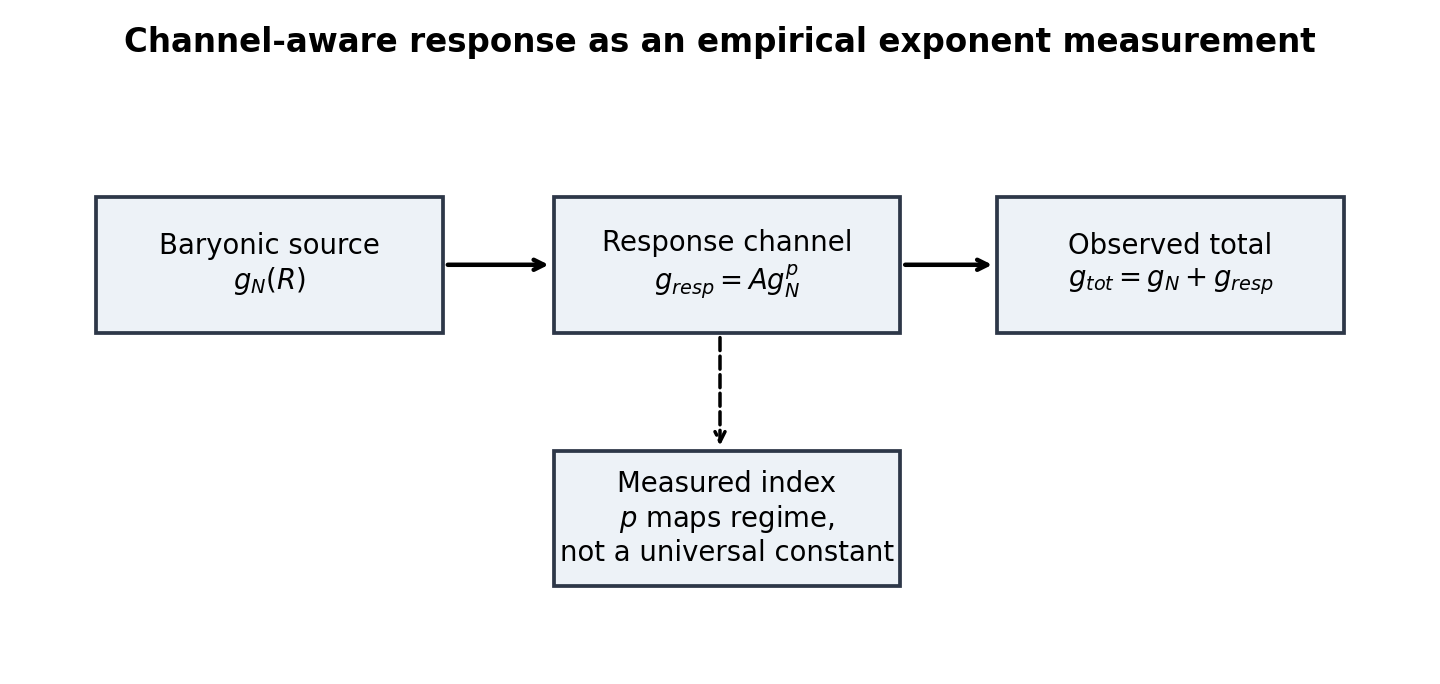
\includegraphics[width=0.92\columnwidth]{figures/fig01_response_channels.png}
\caption{Schematic hierarchy of the channel-aware response idea.  The scalar law tested here is the radial projection of a response-channel model, not the full theory.}
\end{figure}

\section{The fixed GMR prescription}
The fixed GMR prescription is a concrete empirical closure that turns baryonic-geometry quantities into a response operator.  It uses local tidal and curvature information.  Here $T_{ij}=\partial_i\partial_j\phi_B$ is the baryonic tidal tensor and $\|T\|$ is its Frobenius norm.  The scalar $|\nabla^2\phi_B|$ is the magnitude of the baryonic Laplacian; the small floor $\epsilon_A$ carries the same denominator units.  With this convention $A_B$ is a dimensionless local anisotropy measure rather than a new acceleration scale:
\begin{equation}
A_B(R)=\frac{\|T(R)\|}{|\nabla^2\phi_B(R)|+\epsilon_A},
\end{equation}
\begin{equation}
C_B(R)=
\frac{\ell_*|\nabla^2\phi_B(R)|}
{\left[(\partial_R\phi_B)^2+A_*^2+\epsilon_C\right]^{1/2}},
\end{equation}
where $\epsilon_C$ has the dimensions of the squared radial-field term in the bracket.  The bounded local tracer is
\begin{equation}
\nu_B(R)=\frac{A_B(R)+C_B(R)}{1+A_B(R)+C_B(R)} .
\end{equation}
Its non-local state is cumulative:
\begin{equation}
Q_{\rm enc}(R_i)=\sum_{j\le i}\nu_B(R_j)\Delta R_j,
\end{equation}
The radial samples are sorted by increasing $R_i$ before this cumulative state is evaluated; $\Delta R_j$ is the adjacent radial spacing in that ordered profile.  The implementation tested here treats this as a first-order cumulative radial feature, not as a high-order quadrature estimate of a unique continuum integral.  The comparison tests this specific ordered feature and does not claim invariance under alternative radial integration rules.
\begin{equation}
S_\Psi(R_i)=
\frac{Q_{\rm enc}(R_i)}{Q_*+Q_{\rm enc}(R_i)} .
\end{equation}
The response angle and suppression factor are
\begin{equation}
\alpha_B(R_i)=\arctan
\left[
\frac{A_B(R_i)+\eta_S S_\Psi(R_i)}{1+C_B(R_i)}
\right],
\end{equation}
\begin{equation}
S_{\rm rad}(R_i)=
\left[1+\lambda_s\nu_B(R_i)C_B(R_i)\right]^{-1} .
\end{equation}
The response acceleration is
\begin{equation}
g_\chi^{\rm GMR}(R_i)=
\mathcal A_{\rm GMR}\sin\alpha_B(R_i)
\sqrt{g_N(R_i)}S_{\rm rad}(R_i).
\end{equation}
Thus the prescription contains a square-root core but is not identical to a pure square-root law: the factor $\sin\alpha_B S_{\rm rad}$ carries the tested geometric information.  The grid used here has $\mathcal A_{\rm GMR}=1.39458\times10^{-5}$ and $\lambda_s=10.0$.  In the rotation-curve convention used for the calculations, accelerations are stored as $g=V^2/R$ with $V$ in km\,s$^{-1}$ and $R$ in kpc; hence $g$ has units km$^2$\,s$^{-2}$\,kpc$^{-1}$ and $\mathcal A_{\rm GMR}$ has units km\,s$^{-1}$\,kpc$^{-1/2}$.  These values are kept fixed in the external response-exponent comparisons.

\begin{figure}[!htbp]
\centering
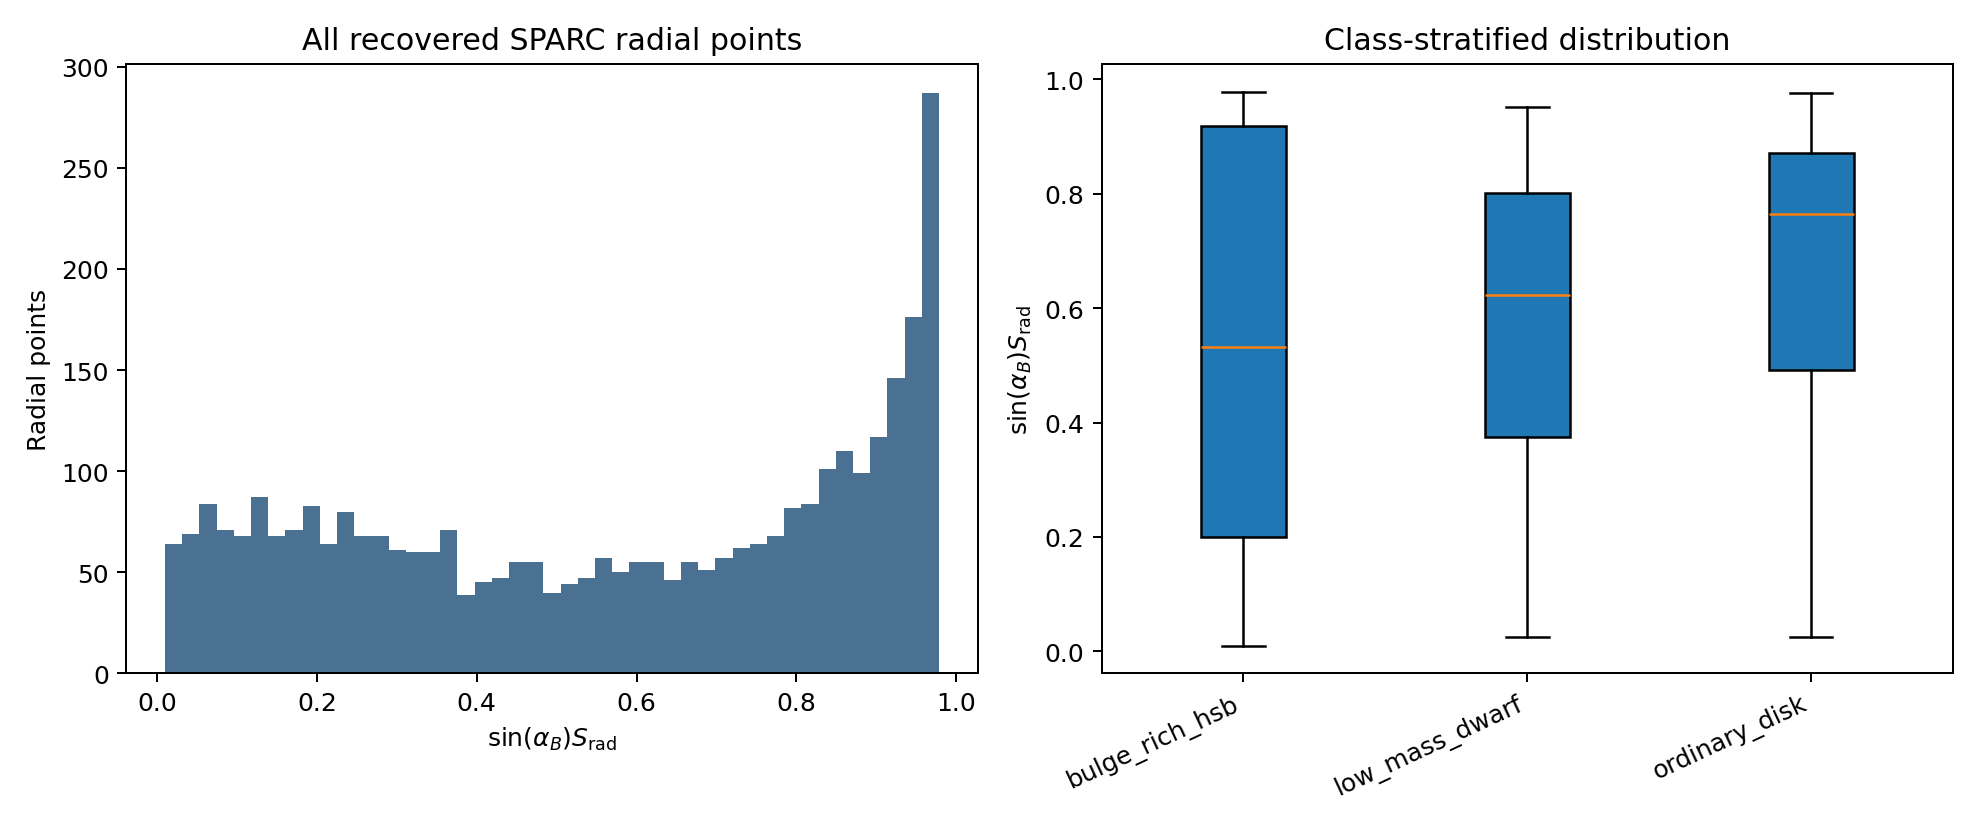
\includegraphics[width=0.92\columnwidth]{figures/fig02_response_modulation.png}
\caption{The GMR modulation factor is not constant.  The fixed prescription contains a square-root core but also tests whether baryonic invariants add predictive information.}
\end{figure}

\section{Data sets and evidence tiers}
The analysis keeps four evidence tiers separate.  SPARC is the primary benchmark.  A public low-surface-brightness sample provides a small but direct component test with explicit gas, disk, and bulge velocities \citep{deBlok2001}.  LITTLE THINGS is used in two more cautious ways: as a proxy based on public total and dark-matter curves, and as a vector-recovered component subset from published mass-model figures \citep{Walter2008THINGS,deBlok2008THINGS,Hunter2012,Oh2015,Iorio2017,Trachternach2008}.

\begin{table}[!htbp]
\centering
\scriptsize
\begin{tabular}{@{}llll@{}}
\toprule
Tier & Data & Input & Role\\
\midrule
Primary & SPARC & mass models & main\\
Direct & LSB & components & external\\
Proxy & LT & $V_{\rm tot}^2-V_{\rm DM}^2$ & stress test\\
Vector & LT & vector-recovered & appendix caveat\\
\bottomrule
\end{tabular}
\caption{Evidence tiers.  Proxy/vector quantities are not official component tables.}
\end{table}

\subsection{Response-exponent estimation}
For a fixed exponent $p$, the projected scalar control is evaluated as $g_{\rm model}=g_N+A_p g_N^p$ and converted to a circular-speed prediction at each tabulated radius.  The displayed comparisons hold two branches fixed: SQRT uses $p=0.5$, while FREEP uses $p\simeq0.298$.  The latter value comes from the OMEGA/SPARC calibration track, where a one-parameter power-law family was scanned under the equal-weight galaxy RMSE objective after fitting the amplitude for each fixed exponent.  Here it serves only as a comparison branch.  It is not re-estimated for each external sample, and no independent physical constant is assigned to it.  Unless a table states otherwise, the objective is the equal-weight galaxy RMSE,
\begin{equation}
{\rm RMSE}_{\rm EW}=\left[\frac{1}{N_{\rm gal}}\sum_g {\rm RMSE}_g^2\right]^{1/2},
\end{equation}
with ${\rm RMSE}_g$ computed from the radial velocity residuals of galaxy $g$.  Observation-weighted RMSE is reported separately where available.  The external comparison table gives fixed-branch tests rather than new per-galaxy free-$p$ fits.  In particular, the phrase ``the $p\simeq0.298$ branch'' denotes a fixed model-comparison branch, not an independent measurement of $p=0.298$ in every data set.

\section{SPARC benchmark}
On the full SPARC sample, the square-root control has an equal-weight RMSE of 40.241 \kms, while fixed GMR gives 40.554 \kms.  On the non-calibration complement, the corresponding values are 41.329 and 41.870 \kms.  The tested GMR invariants do not improve the main equal-weight benchmark beyond the simpler square-root response.

\begin{table}[!htbp]
\centering
\scriptsize
\begin{tabular}{llrrr}
\toprule
Sample & Model & EW & Median & Frac.\\
\midrule
full & GMR & 40.554 & 16.167 & --\\
full & Baryons & 69.316 & 42.879 & 0.886\\
full & MOND & 44.907 & 28.160 & 0.726\\
full & NFW & 46.613 & 8.401 & 0.320\\
full & ISO & 20.316 & 4.919 & 0.074\\
full & Burkert & 25.862 & 5.646 & 0.086\\
held-out & GMR & 41.870 & 16.033 & --\\
held-out & Baryons & 71.026 & 42.879 & 0.874\\
held-out & MOND & 45.366 & 28.352 & 0.715\\
held-out & NFW & 48.450 & 9.307 & 0.338\\
held-out & ISO & 20.869 & 4.770 & 0.079\\
held-out & Burkert & 27.081 & 5.522 & 0.093\\
\bottomrule
\end{tabular}
\caption{SPARC metrics in \kms.  Fraction denotes the share of galaxies for which GMR has a lower RMSE than the listed comparator.  Cored halo baselines remain stronger empirical fits overall \citep{Navarro1996,Navarro1997,Burkert1995,Gentile2004}.}
\end{table}

The SPARC comparison is not a binary success or failure.  In the equal-weight aggregate, the fixed GMR prescription improves on baryons-only, MOND, and reduced NFW.  Galaxy by galaxy, however, reduced NFW retains the smaller median residual and the larger lower-RMSE fraction, while reduced ISO and Burkert remain stronger empirical halo prescriptions overall.  Observation-weighted scoring also changes the ordering: GMR has a full-sample $N_{\rm obs}$-weighted RMSE of 57.334 \kms, whereas MOND gives 52.224 \kms.  The response prescription is best read as a structured constraint on possible baryonic-response terms.  The tabulated RMSE values are point estimates; a complete set of per-model galaxy-bootstrap intervals is not included here.

\begin{figure}[!htbp]
\centering
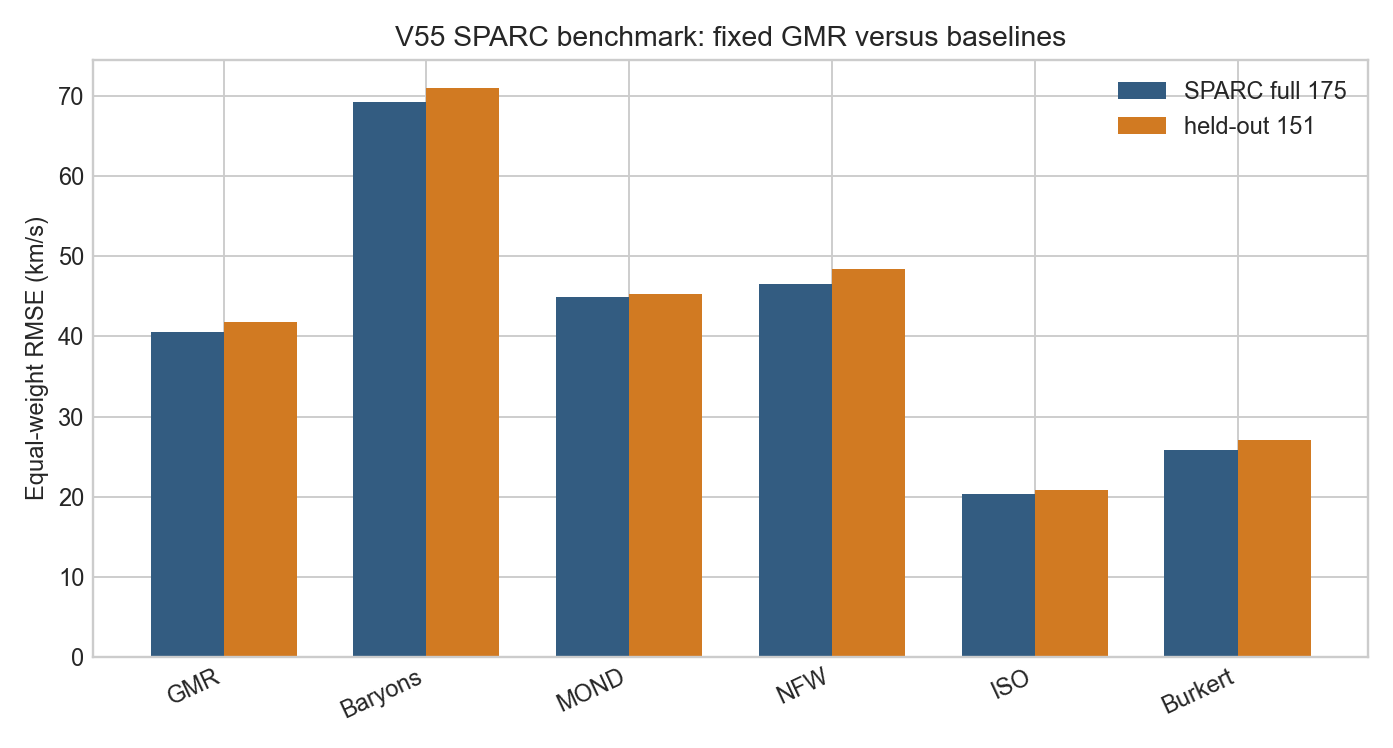
\includegraphics[width=0.92\columnwidth]{figures/fig03_sparc_rmse.png}
\caption{SPARC aggregate comparison.  The fixed response has non-trivial aggregate behavior, but it does not outperform SQRT or the cored halo baselines.}
\end{figure}

\subsection{Ablations and leverage}
The cumulative state variable matters within the GMR family.  Replacing it by a local state gives 47.683 \kms\ on the full sample and 49.398 \kms\ on the held-out subset, substantially worse than the cumulative prescription.  This does not overturn the square-root comparison, but it shows that the cumulative term carries measurable information.

The SPARC aggregate is also leverage-sensitive.  Some large residual improvements occur in a finite set of galaxies, while reduced NFW has lower RMSE for the majority of individual systems.  For that reason the analysis reports aggregate RMSE, median residual, lower-RMSE fractions, observation-weighted metrics, and class stress together.  In the class-stress table, the GMR-over-NFW lower-RMSE fractions are 41/77 for bulge-rich high-surface-brightness systems (0.532; Wilson 95\% interval 0.422--0.640), 11/81 for low-mass dwarfs (0.136; 0.078--0.227), and 4/17 for ordinary disks (0.235; 0.096--0.473).

\begin{figure}[!htbp]
\centering
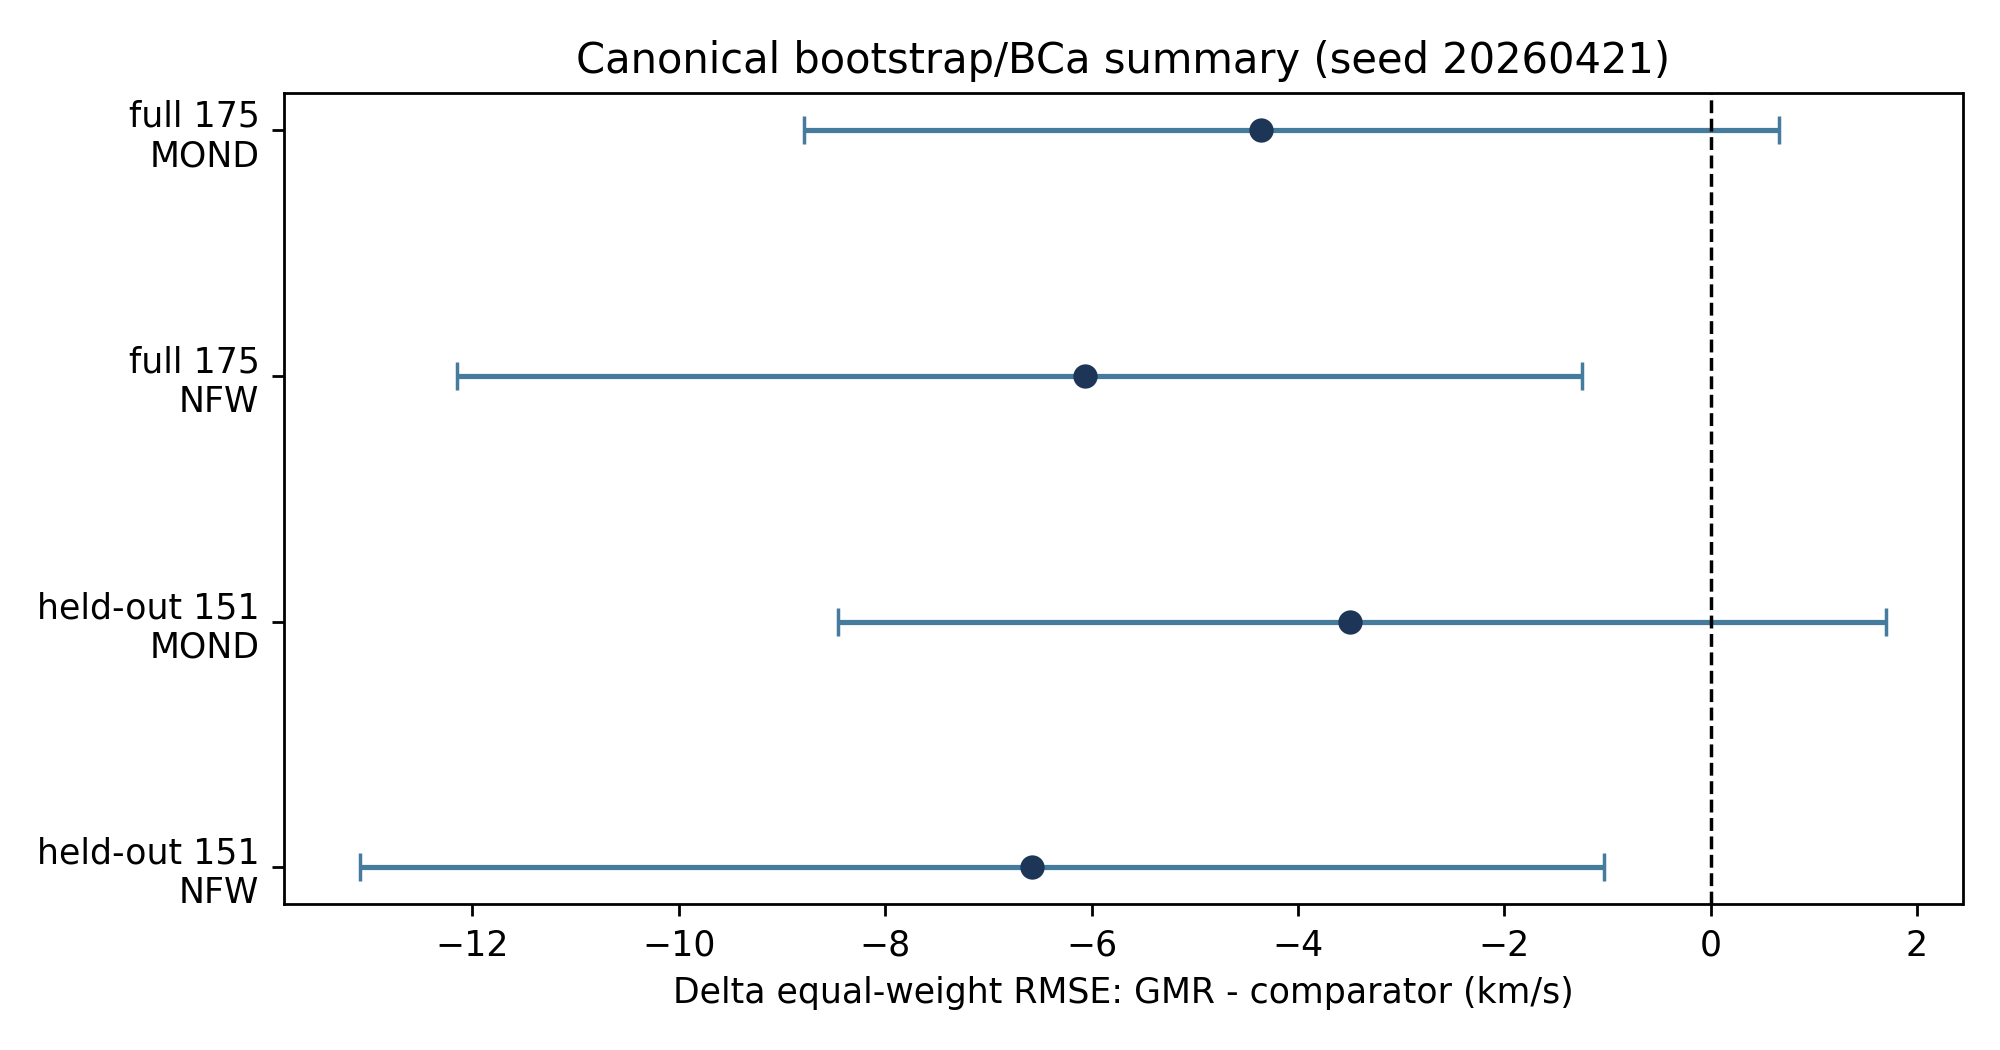
\includegraphics[width=0.92\columnwidth]{figures/fig04_bootstrap_summary.png}
\caption{Bootstrap summary for the fixed SPARC comparisons.  Several effects are descriptive rather than decisive.}
\end{figure}

\section{Residual geometry test at fixed baryonic acceleration}
The most direct empirical test of channel separation is conditional: hold the baryonic acceleration fixed and ask whether baryonic geometry still predicts the residuals.

\subsection{Null scalar-acceleration hypothesis}
The null model is not that all residuals vanish.  Real rotation curves contain distance errors, inclination uncertainties, stellar mass-to-light uncertainty, non-circular motions, gas corrections, and environmental effects \citep{Trachternach2008,BellDeJong2001,Chabrier2003,Meidt2014,Courteau2014}.  The stricter and testable null is instead conditional: after a flexible one-variable acceleration law has accounted for $\log g_{\rm bar}$, the remaining residuals are expected not to show an additional systematic dependence on baryonic structural invariants.  That null is modeled with a cubic RAR baseline,
\begin{equation}
\log_{10}g_{\rm obs}=a_0+a_1 z+a_2 z^2+a_3 z^3+\epsilon,
\end{equation}
where $z$ is standardized $\log_{10}g_{\rm bar}$.  This flexible scalar baseline is designed to absorb the main RAR curvature before any residual geometry term is tested.

\subsection{GMR response-channel prediction}
In GMR, the observable acceleration is the projection of distinct baryonic-source and response channels rather than a single scalar function of $g_{\rm bar}$.  The parent geometry is
\begin{equation}
g_{\rm obs}^2=g_N^2+g_\chi^2+2\kappa g_Ng_\chi ,
\end{equation}
with $g_\chi=A_\chi g_N^p$ and $\kappa=\cos\theta_{\rm int}$.  If the response amplitude or alignment depends on baryonic geometry, then two points with the same $g_N$ need not have identical projected acceleration.  To first order, the residual around a one-variable scalar law can be written schematically as
\begin{equation}
\delta\log g_{\rm obs}
\simeq
\frac{\partial\log g_{\rm obs}}{\partial \kappa}\delta\kappa(I_B)
+
\frac{\partial\log g_{\rm obs}}{\partial \log A_\chi}\delta\log A_\chi(I_B),
\end{equation}
where $I_B$ denotes baryonic structural information.  In the fixed GMR prescription, the intended invariants are the baryonic anisotropy and curvature tracers $A_B$ and $C_B$, together with their cumulative state.  In the raw SPARC test below, observable compactness/profile proxies are used for the same question because SPARC does not provide all three-dimensional baryonic invariants directly.

The geometry-augmented model then adds a Fisher-length summary of baryonic compactness/profile variables,
\begin{equation}
\log_{10}g_{\rm obs}=f_3(\log_{10}g_{\rm bar})+
\beta_i L_{B,i}+\epsilon.
\end{equation}
The profile vector entering $L_B$ uses only baryonic/profile quantities: disk and bulge surface-brightness logs, $R/R_{\rm disk}$, $R/R_{\rm eff}$, and local slopes/curvatures of the baryonic acceleration and disk surface-brightness profiles.  It does not use $V_{\rm obs}$ or the rotation-curve residuals to construct the predictors.  SPARC does not provide a direct vertical disk-thickness observable, so this test probes compactness and radial-profile structure rather than physical disk thickness.

\subsection{SPARC MCMC test}
The MCMC uses four chains, 14,000 steps per chain, a 5,000-step burn-in, and thinning by five, following the affine-invariant ensemble-sampling approach \citep{GoodmanWeare2010,ForemanMackey2013}.  Wide Gaussian priors are placed on standardized coefficients, with an uninformative bounded prior on $\log\sigma$.  The maximum $\hat R$ values are 1.010 for the cubic baseline and 1.007 for the geometry model.

\begin{table}[!htbp]
\centering
\scriptsize
\begin{tabular}{lrr}
\toprule
Quantity & Value & Meaning\\
\midrule
$N_{\rm point}$ & 3389 & SPARC radial points\\
$N_{\rm gal}$ & 175 & galaxies\\
RMSE cubic RAR & 0.19438 dex & in-sample\\
RMSE + geometry & 0.19125 dex & in-sample\\
$\Delta$RMSE & 0.00313 dex & positive but small\\
CV $\Delta$RMSE & 0.00218 dex & galaxy-fold cross-validation\\
$\Delta$BIC & $-85.6$ & point-level, favors geometry\\
\bottomrule
\end{tabular}
\caption{Residual-geometry MCMC summary.  Negative $\Delta$BIC favors the geometry-augmented model, but the point-level BIC is interpreted cautiously because radial points within a galaxy are correlated.}
\end{table}

A direct-proxy diagnostic gives the same direction.  Adding the raw standardized profile proxies instead of the Fisher-length compression gives $\Delta{\rm BIC}=-91.4$ relative to the cubic baseline, with maximum $\hat R=1.026$.  The largest posterior coefficients by absolute median are $R/R_{\rm disk}$, disk surface brightness, and $R/R_{\rm eff}$.  These direct-proxy coefficients are treated as descriptive rather than physical, because the profile variables are mutually correlated and are not independent measurements of a unique three-dimensional geometry.

The point-level result is supported by a galaxy-block check.  After subtracting the cubic RAR baseline and averaging residuals by galaxy, the posterior coefficient of the total baryonic-profile Fisher length is positive: $\beta_{L_B}=0.0389$ dex per standardized unit, with a 95\% credible interval $[0.0106,0.0673]$ and $P(\beta_{L_B}>0)=0.996$.  This is the most direct evidence in the present paper that baryonic-profile geometry can carry residual information at fixed $g_{\rm bar}$.

\begin{figure}[!htbp]
\centering
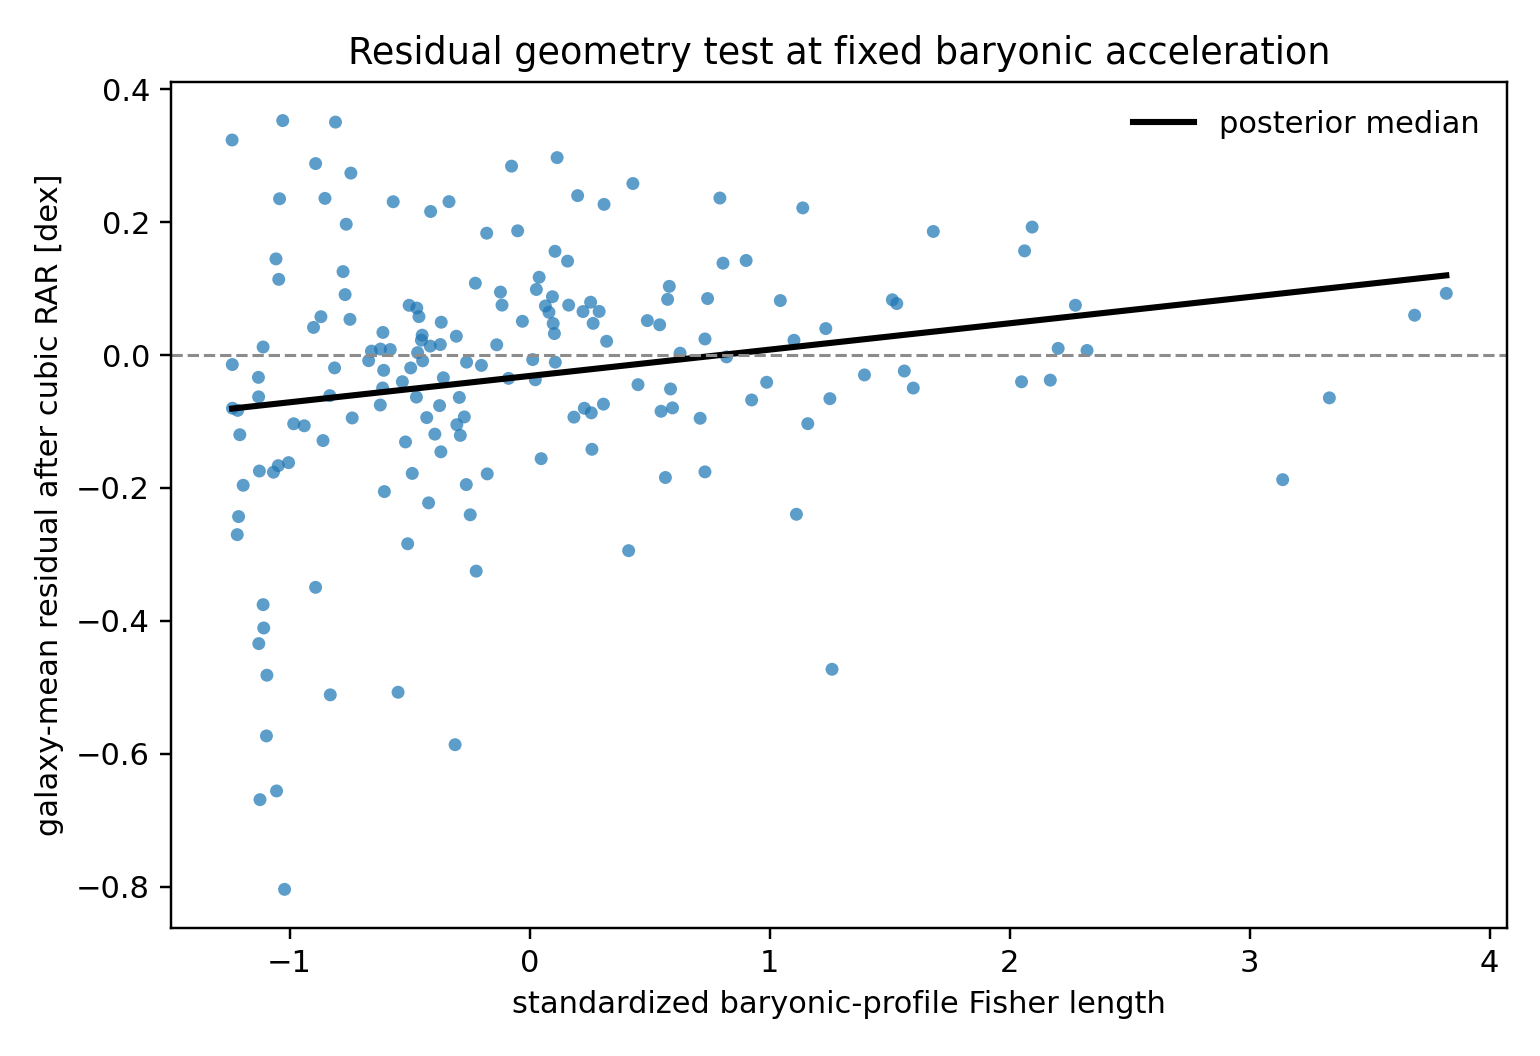
\includegraphics[width=0.92\columnwidth]{figures/fig05_residual_geometry_mcmc.png}
\caption{Galaxy-block residual-geometry test.  The horizontal axis is the standardized total Fisher length of the baryonic compactness/profile vector.  The vertical axis is the galaxy-mean residual after removing a cubic one-variable RAR baseline.}
\end{figure}

\subsection{Open validation}
The interpretation is intentionally limited.  The RMSE gain is small, SPARC does not provide a direct disk-thickness degree of freedom, and the test does not derive a covariant response law.  Its value is that it identifies a measurable candidate discriminator.  If independent data show no residual dependence on baryonic geometry at fixed $g_{\rm bar}$, the present GMR interpretation reduces to a one-variable MOND/RAR projection.  If the residual-geometry signal strengthens under independent component tables and no-retuning validation, it becomes the most direct empirical route by which GMR can separate itself from MOND/AQUAL/QUMOND phenomenology.

\subsection{Oh-supplied component-table residual-geometry check}
\label{subsec:oh-direct-geometry}

The SPARC residual-geometry test is complemented by an independent component-table check using LITTLE THINGS/THINGS rotation-curve tables provided by S.-H. Oh.  For the LITTLE THINGS systems, the asymmetric-drift-corrected velocity column recommended by Oh is used; for IC~2574, $V_{\rm rot}$ is used, following the data note.  Only derived quantities enter the present analysis.  The author-supplied machine-readable tables are not redistributed.

The null model contains galaxy fixed effects, $\log_{10}g_N$, and a relative radial coordinate.  The geometry model adds three pre-specified baryonic-channel summaries: a normalized baryonic Fisher-length proxy $L_B$, the local gas contribution fraction $p_{\rm gas}$, and the radial profile-gradient term $dL_B/d\ln R$.  The test is deliberately narrow: after controlling for the one-variable acceleration law and for galaxy identity, does baryonic geometry or composition still predict residual acceleration?

The component subset favors the geometry-augmented model.  On the full component subset, the test uses 26 galaxies and 877 radial points and improves the Bayesian information criterion from ${\rm BIC}=390.51$ to ${\rm BIC}=346.20$, or
\begin{equation}
\Delta{\rm BIC}_{\rm geom-null}=-44.31 .
\end{equation}
On the predefined quality-control subset excluding DDO~43 and DDO~47, the result strengthens to 24 galaxies and 834 radial points, with
\begin{equation}
\Delta{\rm BIC}_{\rm geom-null}=-92.12 .
\end{equation}
Block bootstrap, permutation, posterior-sign, and leave-one-galaxy-out checks support the dominant composition/profile terms \citep{Efron1979,EfronTibshirani1993,Wilcoxon1945,Wilson1927}.  In the quality-control subset the gas-fraction coefficient is negative with posterior probability $P(\beta_{p_{\rm gas}}<0)=1.000$ in the numerical draw, and the profile-gradient coefficient has $P(\beta_{dL_B/d\ln R}<0)=1.000$.  The scalar $L_B$ coefficient alone is not stable enough to carry the interpretation: its bootstrap interval crosses zero and it is not used as the whole signal.

This is the clearest empirical support for the channel-separation interpretation in the present paper.  It indicates that residuals at fixed $g_N$ are not fully described by a one-variable RAR in this component subset.  It does not, however, derive the response law, the acceleration scale, the lensing sector, the Solar-System limit, or a relativistic closure.


\section{RAR, BTFR, and failure modes}
The RAR and BTFR diagnostics are used only as within-sample consistency checks.  The binned RAR curve gives a log-space RMSE of 0.0640 for fixed GMR, but it is not a literature-level comparison against optimized acceleration-law implementations.  The BTFR proxy slope is 3.687 against an observed 3.486, with broader scatter, 0.285 dex rather than 0.225 dex.  Thus the prescription is slope-consistent but not scatter-matching.

\begin{figure}[!htbp]
\centering
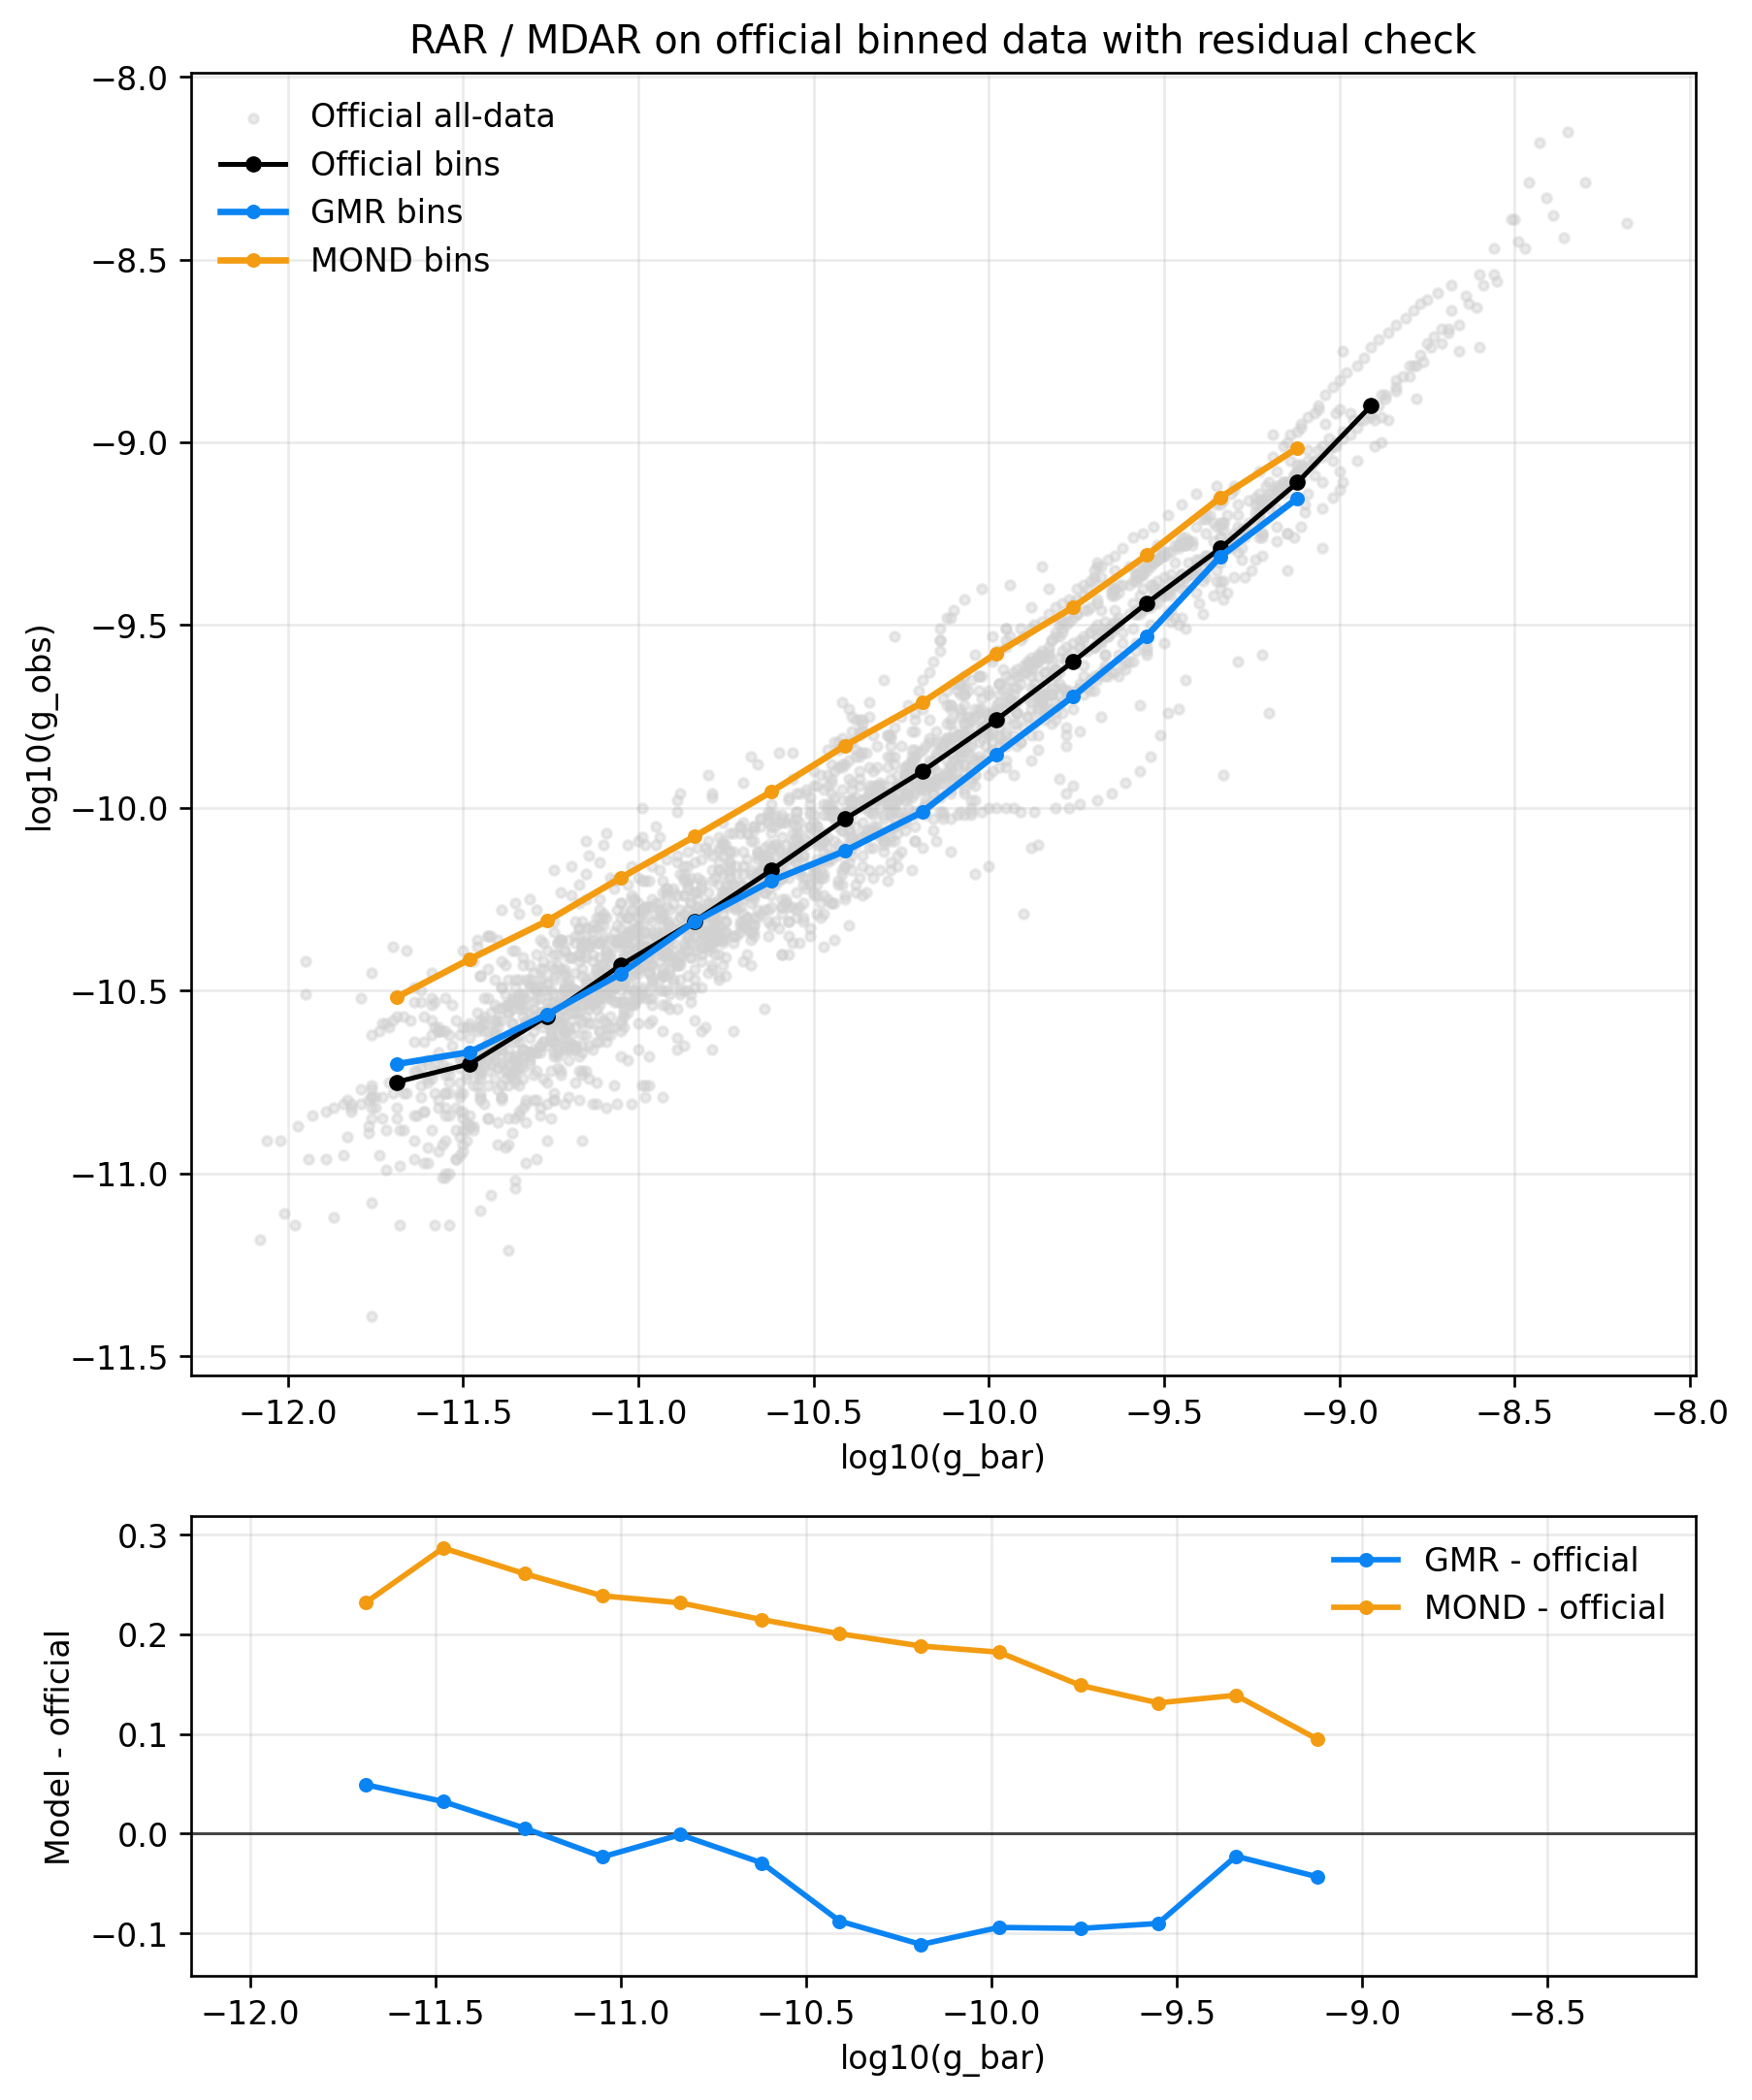
\includegraphics[width=0.92\columnwidth]{figures/fig06_rar.png}
\caption{Binned RAR diagnostic used as a within-sample consistency check.}
\end{figure}

\begin{figure}[!htbp]
\centering
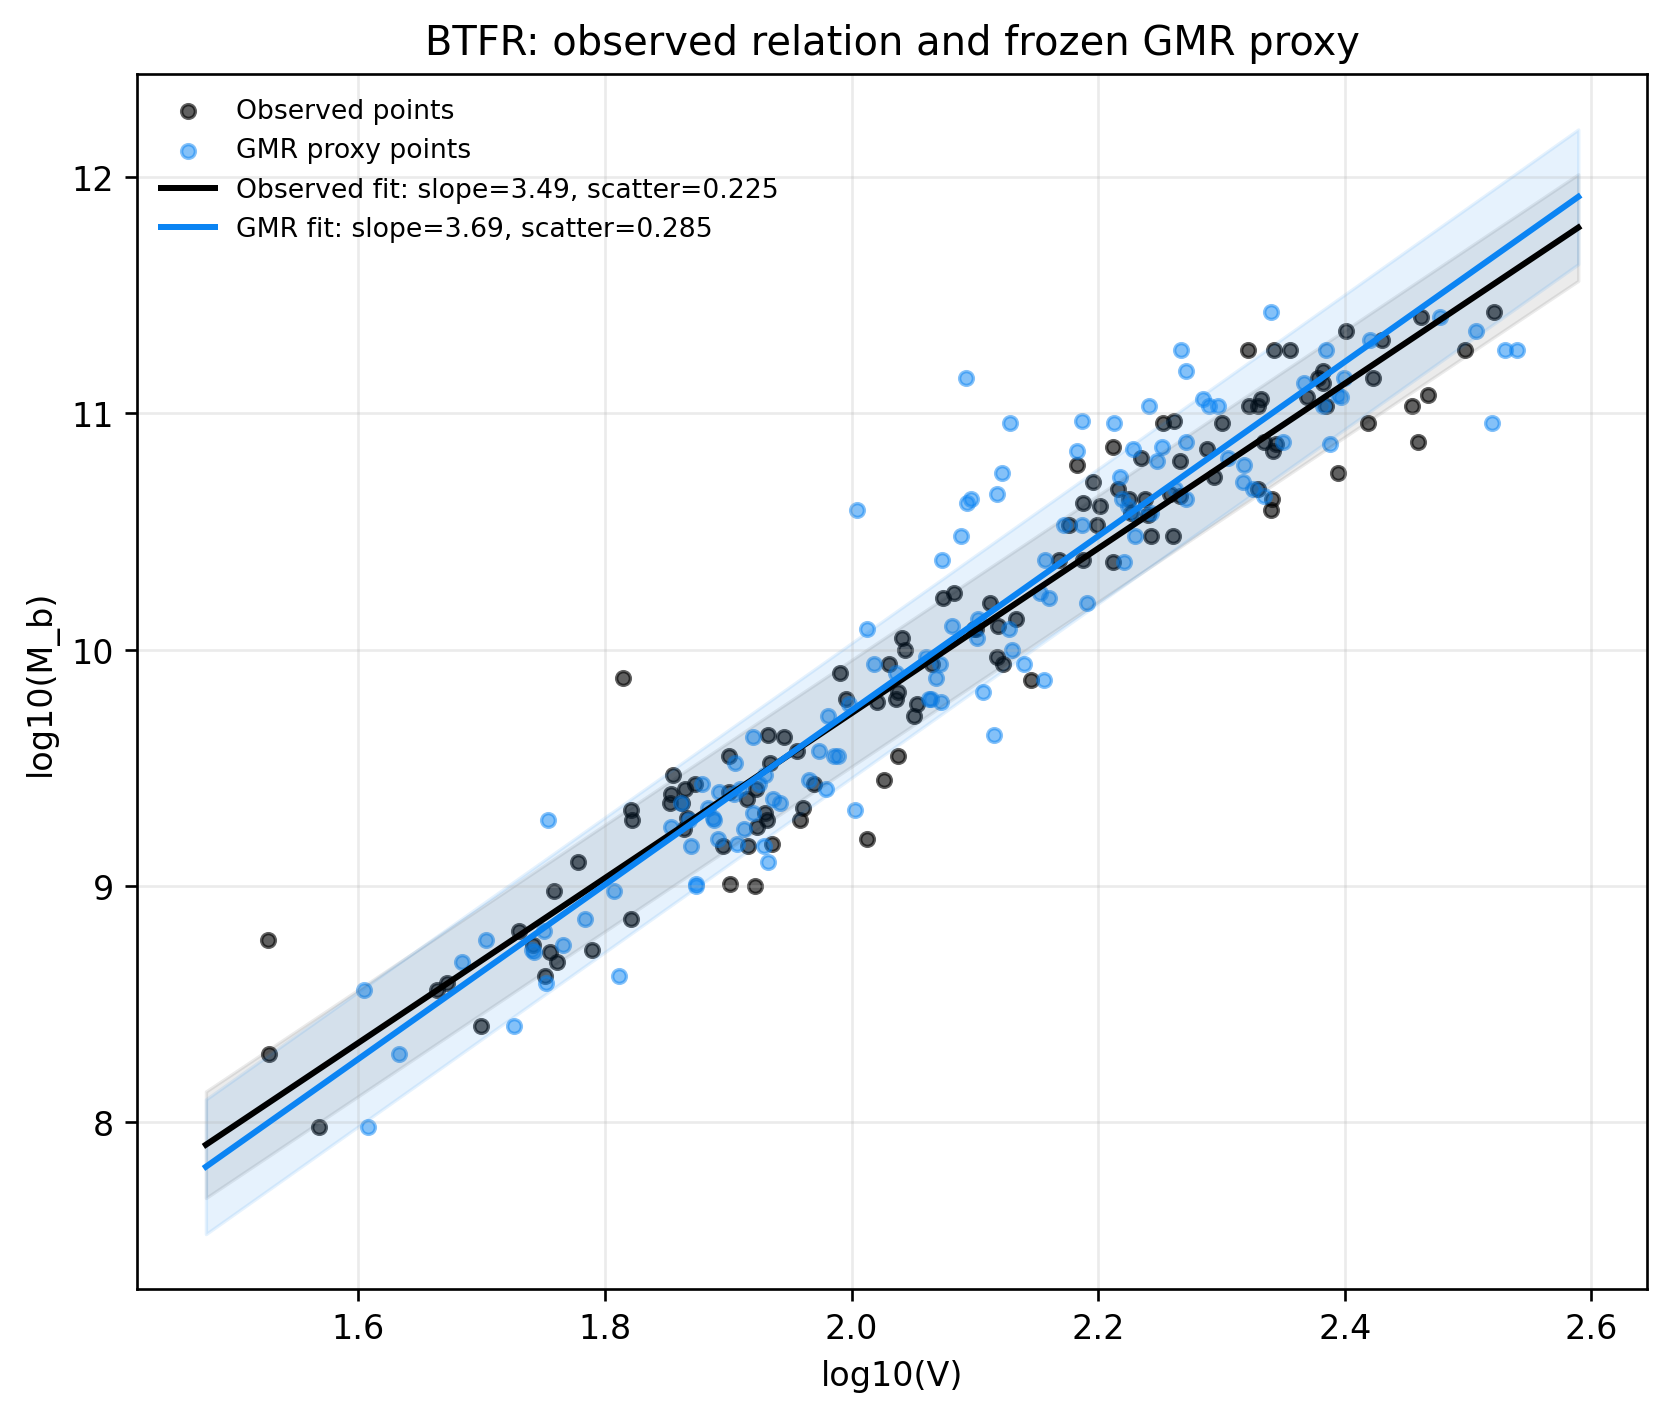
\includegraphics[width=0.92\columnwidth]{figures/fig07_btfr.png}
\caption{BTFR diagnostic.  The proxy is slope-consistent but broader in scatter than the observed relation.}
\end{figure}

The clearest weakness of the fixed GMR prescription is the low-mass dwarf and low-surface-brightness regime, where diversity, feedback, and halo-core systematics are already known to be important \citep{Swaters2009,Oman2015,BullockBoylanKolchin2017,PontzenGovernato2012,DiCintio2014,Read2016,Katz2017}.  In the low-mass-dwarf slice, GMR has an RMSE of 15.523 \kms, while reduced NFW and ISO give 6.880 and 4.478 \kms.  Ordinary disks remain difficult, and several high-leverage failures are not dwarfs, so the failure mode is primary rather than exclusive.

\section{Response exponent across regimes}
The exponent comparison is deliberately conservative.  SPARC equal-weight metrics and the direct LSB component sample favor the fixed $p\simeq0.298$ branch, while LITTLE THINGS proxy tests and the validated vector-recovered subset lean toward $p=0.5$.  The rows below are fixed-branch comparisons rather than per-galaxy exponent fits: SQRT fixes $p=0.5$, FREEP fixes $p\simeq0.298$ from the calibration track, and the quoted objective is equal-weight per-galaxy RMSE unless stated otherwise.  Because the external evidence combines direct component tables, proxy curves, and vector-recovered components, it cannot yield a single robust posterior interval for a universal $p$.  A full per-data-set fit of $(A_p,p)$ with uncertainty propagation is required before the exponent can be treated as separately measured in each regime.

\begin{table}[!htbp]
\centering
\scriptsize
\begin{tabular}{lrrrrl}
\toprule
Data & $N$ & SQRT & FREEP & Fav. & Status\\
\midrule
SPARC full & 175 & 40.241 & 39.085 & FREEP & calibration\\
SPARC hold. & 151 & 41.329 & 40.322 & FREEP & calibration\\
LSB direct & 8 & 18.772 & 16.607 & FREEP & small N\\
LT proxy drop & 22 & 17.622 & 18.487 & SQRT & proxy\\
LT proxy clamp & 22 & 17.791 & 18.615 & SQRT & proxy\\
LT vector & 17 & 16.446 & 16.570 & SQRT & weak\\
\bottomrule
\end{tabular}
\caption{Response-exponent evidence map.  RMSE values are in \kms.  The vector-recovered LITTLE THINGS row is directional, not decisive.}
\end{table}

\begin{figure}[!htbp]
\centering
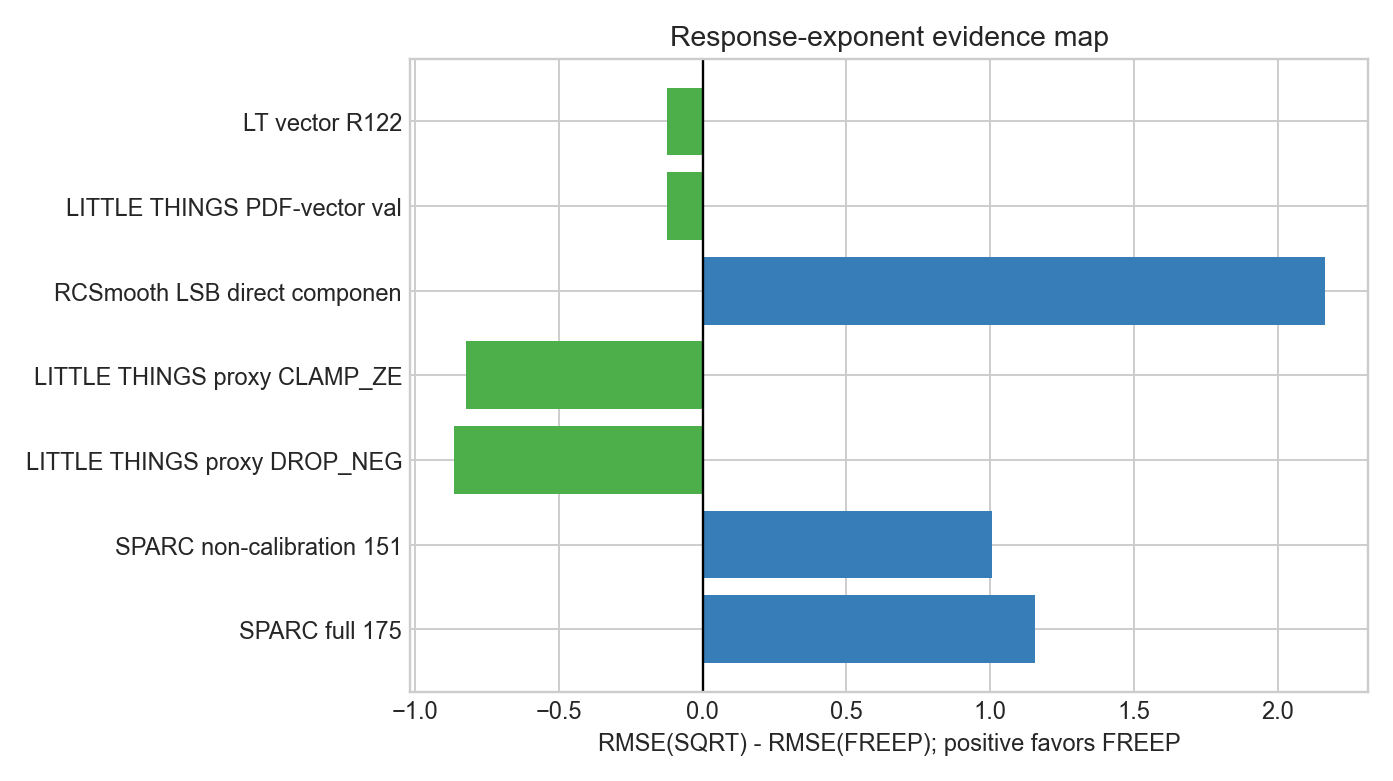
\includegraphics[width=0.92\columnwidth]{figures/fig08_response_evidence_map.png}
\caption{Dataset dependence of SQRT versus FREEP.  Positive values favor FREEP; negative values favor SQRT.}
\end{figure}

\begin{figure}[!htbp]
\centering
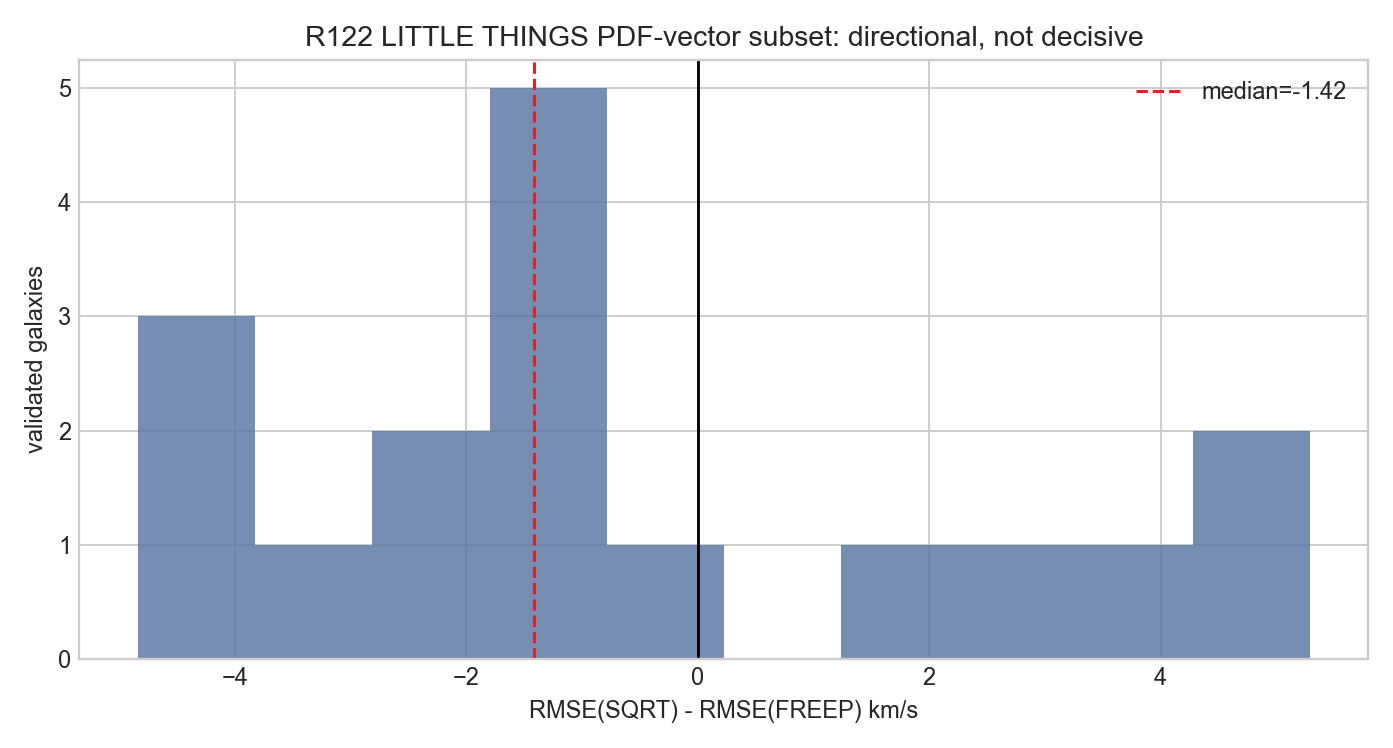
\includegraphics[width=0.92\columnwidth]{figures/fig09_little_things_delta_histogram.png}
\caption{Per-galaxy delta distribution for the validated vector-recovered LITTLE THINGS subset.  SQRT has a small but statistically weak edge.}
\end{figure}

The vector-recovered subset is treated conservatively.  Seventeen galaxies pass validation, including fifteen GOLD and two SILVER cases.  The validation gate is independent of the SQRT/FREEP comparison: accepted cases reproduce the published reference curves well enough to be used, while rejected cases either fail that check or lack a matched dark-matter curve.  SQRT has lower RMSE in eleven of the seventeen, with 16.446 \kms\ versus 16.570 \kms\ for FREEP.  A paired sign test gives $p=0.332$; a galaxy-resampling bootstrap for the aggregate SQRT-minus-FREEP RMSE difference gives a 95\% interval of $[-1.76,+1.36]$ \kms\ and $P(\Delta<0)=0.609$.  This is a weak directional result.  It is consistent with the LITTLE THINGS proxy split, but it is too small and too uncertain to support a universal law.  Rejected galaxies are left outside the sample.

\section{Compact transition prescription}
\label{sec:master-transition}

The branch comparison leaves a useful tension.  Asymptotically flat rotation curves and the baryonic Tully-Fisher relation require a square-root response, whereas the finite-radius SPARC and direct LSB comparisons prefer a shallower projected branch near $p\simeq0.30$.  This section uses a compact transition family as an empirical description of the projected scalar branch,
\begin{equation}
g_\chi^{\rm MF}(g_N;q,s,N)=
\sqrt{a_0g_N}
\left[1+\left(N\,\frac{g_N}{a_0}\right)^s\right]^{-q}.
\label{eq:gmr-mf-family}
\end{equation}
Here $a_0$ is the usual empirical acceleration scale, $N=a_0/g_c$ sets the transition location, and $(q,s)$ control the width and slope of the finite-radius departure from the square-root branch.  The local logarithmic slope is exactly
\begin{equation}
p_{\rm eff}(g_N)
=\frac{d\ln g_\chi^{\rm MF}}{d\ln g_N}
=\frac{1}{2}
-q\,s\,
\frac{x^s}{1+x^s},
\qquad
x\equiv N\,\frac{g_N}{a_0}.
\label{eq:peff-general}
\end{equation}
The useful mathematical point is the closed expression for $p_{\rm eff}$: a square-root asymptote can coexist with a finite-radius window in which the projected response appears shallower.

The fiducial benchmark used in the figures and summary tables is
\begin{equation}
q=0.15,\qquad s=1.50,\qquad N=144,
\end{equation}
or
\begin{equation}
g_\chi^{\rm MF}(g_N)=
\sqrt{a_0g_N}
\left[1+\left(144\,\frac{g_N}{a_0}\right)^{3/2}\right]^{-3/20}.
\label{eq:gmr-mf}
\end{equation}
For the adopted acceleration windows this benchmark gives a mean finite-disk value $p_{\rm eff}=0.2996$ and a low-acceleration value $p_{\rm eff}=0.4945$.  This is the precise meaning assigned here to the $p\simeq0.30$ branch: it is a projected finite-radius response window, not a universal asymptotic law.

The numerical values in Eq.~(\ref{eq:gmr-mf}) are interpreted conservatively.  The inverse search used a grid with steps $\Delta q=0.01$ and $\Delta s=0.02$, so the rational appearances $q=3/20$ and $s=3/2$ are not by themselves physical derivations.  In addition, the value $s=1.50$ lies on the upper boundary of the scan and requires a wider scan before any structural interpretation is attached to it.  The fiducial $N=144$ is a compact benchmark close to the scanned transition scale, but nearby integer or cosmological normalizations can give comparable numerical proximity.  A normalization near the inverse fine-structure constant, $\alpha^{-1}\simeq137.036$ \citep{CODATA2022Constants}, is theoretically intriguing for future vacuum-polarization interpretations, but the direct $a_0/N$ comparison used here favors $N\simeq144$ over $N\simeq137$, and no electromagnetic or quantum-vacuum sector is derived in this work.  No claim is made here that this benchmark follows from a primitive counting rule.

It is sometimes useful to introduce a response-eigenvalue notation.  If a radial projection factor is denoted $C(g_N)$ and one defines $C=H_R^{-3/4}$, then Eq.~(\ref{eq:gmr-mf-family}) is equivalent to
\begin{equation}
H_R(g_N)=
\left[1+\left(N\,\frac{g_N}{a_0}\right)^s\right]^{4q/3}.
\end{equation}
This is an algebraic reparameterization, not a derivation of $H_R$ from an action.  A future covariant theory would have to derive $H^{\mu\nu}[I_B]$, $a_0$, $N$, $q$, and $s$ from its field equations rather than defining them to reproduce Eq.~(\ref{eq:gmr-mf-family}).


\section{Relation to MOND, AQUAL, and QUMOND}
The square-root branch is treated as part of the MOND family of phenomenology, not as independent evidence for a new theory.  In the deep-acceleration limit of MOND, $g_{\rm obs}\simeq (a_0g_N)^{1/2}$, which gives asymptotically flat rotation curves and the baryonic Tully-Fisher scaling \citep{Milgrom1983,FamaeyMcGaugh2012}.  AQUAL provides a nonrelativistic Lagrangian realization of this scaling and an external-field effect \citep{BekensteinMilgrom1984}; QUMOND rewrites the same phenomenology in a quasi-linear form \citep{Milgrom2010QUMOND}.  Relativistic completions such as TeVeS and later MOND-inspired models show that this step is nontrivial and cannot be replaced by a scalar rotation-curve fit alone \citep{Bekenstein2004,SkordisZlosnik2021}.

The same constraint appears directly in the response-exponent language.  For a point-like baryonic source in the response-dominated outer regime,
\begin{equation}
 \frac{V^2(R)}{R}\simeq A\left(\frac{GM_b}{R^2}\right)^p ,
\end{equation}
so that
\begin{equation}
 V^2(R)\simeq A G^p M_b^p R^{1-2p}.
\end{equation}
Asymptotically flat rotation curves require $1-2p=0$, hence $p=1/2$, and then $V^4\propto M_b$.  Therefore the fixed $p\simeq0.298$ branch used above cannot be interpreted as a universal deep-asymptotic law.  Its allowed status is narrower: it is a finite-radius projected comparison branch under the stated metric and data calibration.  If future free-exponent fits show a robust departure from $p=1/2$, they would also need to explain why the outer velocities remain flat.

In the deep asymptotic scaling, the present GMR implementation deliberately overlaps MOND/QUMOND.  Its possible distinct content lies only in whether the baryonic-invariant factors $\sin\alpha_BS_{\rm rad}$ add predictive information beyond a one-variable MOND/RAR relation at fixed $g_N$.  The residual-geometry MCMC above is a first positive but small version of this test: baryonic compactness/profile Fisher length carries residual information after controlling for $g_{\rm bar}$.  A clean discriminator would require the signal to survive independent component tables, no per-galaxy retuning, explicit galaxy-block validation, and direct comparison with AQUAL/QUMOND external-field implementations.

\section{Relativistic gate status}
\label{sec:relativistic-gate-status}

The compact transition law is a galaxy-scale projected response prescription, not a relativistic closure.  Candidate embeddings were checked in scalar, conformal, disformal, vector-tensor, and anisotropic-response families.  The only GMR-specific route that survives as a candidate keeps the tensor kinetic sector Einstein-Hilbert, so that the gravitational-wave speed can remain luminal by construction in the sense required after GW170817/GRB~170817A \citep{Abbott2017GW170817,Abbott2017MultiMessenger,CreminelliVernizzi2017,EzquiagaZumalacarregui2017}, and places the finite-radius response in a scalar/an\-isotropic metric sector.  This is a candidate embedding rather than a closed theory.  The lensing potentials $\Phi$ and $\Psi$, Solar-System/PPN screening, full stability conditions, and the covariant derivation of $H^{\mu\nu}[I_b]$ remain open.  No gravitational-wave, PPN, or cluster-lensing success claim is made in this paper.


\section{Interpretation}
The fixed-branch comparisons suggest regime sensitivity in the projected response branch, although they stop short of measuring that sensitivity as a physical parameter.  The same one-parameter projection behaves differently in SPARC, direct LSB mass models, LITTLE THINGS proxy curves, and vector-recovered dwarf-galaxy components.

A channel-aware interpretation is compatible with this behavior, but the data alone cannot establish it.  A projected exponent can absorb baryonic structure, gas dominance, stellar mass-to-light assumptions, response alignment, and metric weighting.  A deeper theory may still contain a more restrictive exponent; the present evidence has not isolated it.

\section{Limitations and falsifiability}
The scope is narrower than a dark-sector solution.  Cluster lensing, cosmology, Solar-System screening, and a closed action are outside the present analysis.  The LITTLE THINGS component curves used here are vector-recovered from published figures; the CDS tables do not provide separate official $V_{\rm gas}/V_{\rm disk}/V_{\rm bulge}$ component curves.  The direct LSB sample is small; the SPARC free-exponent result is calibration-dependent and metric-dependent; the RMSE tables lack a full galaxy-bootstrap interval for every comparator; and the summary lacks a full error-weighted $\chi^2$ reanalysis.  The cumulative $Q_{\rm enc}$ feature is also a first-order ordered radial sum, not a grid-invariant continuum functional.

The channel-aware equations are a nonrelativistic phenomenological parent, not a completed relativistic gravity theory.  Any completion would need to satisfy post-Newtonian and Solar-System constraints, including Cassini-level bounds, and provide screening or decoupling before the same response law is extrapolated outside galaxy rotation curves \citep{Bertotti2003,Will2014LRR,KhouryWeltman2004}.  The decisive empirical test is to replicate the Oh-supplied no-retuning comparison on additional independently published or independently supplied component tables, ideally with homogeneous uncertainty modeling.  A stronger statistical treatment would also include the full fixed-exponent scan, error-weighted residual metrics, and bootstrap intervals for the principal RMSE comparisons.

The open theoretical requirements are explicit.  First, a covariant action or closed field equation would be needed, with a conservation law compatible with the Bianchi identities.  Second, the acceleration scale and any response amplitude would need to be derived from the model rather than calibrated from the same rotation-curve phenomenology they are intended to explain.  Third, the projection factor or environmental response that would control external-field sensitivity would need to be obtained from one law and then tested on classical dwarf spheroidals without per-object retuning.  Fourth, the lensing potentials $\Phi$ and $\Psi$, the slip parameter, and the effective growth and lensing functions would need to be defined before cluster lensing, weak lensing, CMB, BBN, or large-scale-structure claims can be made \citep{Markevitch2004,Clowe2006,Planck2018Cosmology}.  Finally, a discriminator from AQUAL/QUMOND would need to be specified and tested.  Failure of any of these requirements would leave GMR at the level of an empirical response parameterization.

\section{Data availability}

This study uses published SPARC, LITTLE THINGS, and LSB rotation-curve material.  The original survey files remain in their public archives and are cited through the source papers.  The additional LITTLE THINGS/THINGS component tables supplied by S.-H. Oh are treated as author-supplied source tables for validation; those raw files are not redistributed.  Only derived summary quantities, validation flags, and aggregate statistics needed to reproduce the claims in this paper are included in the accompanying analysis material.  Public reuse of the original component tables requires either permission from the data author or reconstruction from the published source material.


\section{Conclusions}

The fixed GMR prescription defines a baryonic-invariant response architecture with an explicit square-root core.  Its tested invariants do not improve the main SPARC equal-weight RMSE beyond a pure square-root control.  They do, however, make the cumulative-state version substantially better than a local-state ablation and keep the comparison informative against baryons-only, MOND, and reduced NFW baselines.  Cored halo models remain stronger overall, and the dwarf/LSB regime remains the principal empirical stress test.

The main additional result is the residual-geometry check at fixed baryonic acceleration.  In the Oh-supplied LITTLE THINGS/THINGS component subset, baryonic composition and radial profile-gradient terms improve a galaxy-fixed RAR baseline by $\Delta{\rm BIC}=-44.31$ on the full component subset and by $\Delta{\rm BIC}=-92.12$ on the quality-control subset.  This supports the channel-separation idea in a restricted but testable sense: in these data, the rotation curve contains residual information beyond a single scalar function of $g_N$.  The signal is not simply a stand-alone $L_B$ coefficient; the most stable terms are gas fraction and profile-gradient geometry.

The compact transition prescription in Eq.~(\ref{eq:gmr-mf}) gives a controlled way to reconcile the finite-radius $p\simeq0.30$ response window with the required square-root asymptote.  It is used here as an empirical prescription and as a target for theory building, not as a completed derivation.  The benchmark $N=144$ is retained as a fiducial empirical transition normalization; it is not unique and is not evidence that the scale follows from first principles.

The construction is best described as an empirical response framework with a sharpened theoretical target.  A self-consistent physical model would still need to derive the response law, the acceleration scale, the external-field behavior, the relativistic/lensing sector, and a clean MOND/QUMOND discriminant from one closed set of equations.  These are the next theoretical requirements, not results of the present paper.


\section*{Acknowledgments}
\noindent
The author thanks S.-H. Oh for providing the THINGS and LITTLE THINGS rotation-curve files used for the independent component-table check, and for clarifying the recommended use of the asymmetric-drift-corrected velocities for LITTLE THINGS and $V_{\rm rot}$ for IC~2574.  The author thanks D. A. Hunter for routing the LITTLE THINGS component-table query to S.-H. Oh.  The author thanks S. S. McGaugh, F. Lelli, and J. Schombert for correspondence on SPARC, LSB, and LITTLE THINGS data provenance, including cautions about heterogeneous rotation-curve uncertainties and the appropriate use of public mass-model tables.  The author also thanks P. Kroupa for correspondence that sharpened the self-consistency and dwarf-spheroidal/external-field requirements that motivate the cautious framing of this work.  Responsibility for the analysis and interpretation rests with the author.


\appendix
\section{Vector-recovered LITTLE THINGS validation subset}
The LITTLE THINGS vector-recovered check uses 17 accepted galaxies.  For each system, the accompanying table gives the validation class, the number of radial points, and the SQRT/FREEP RMSE values entering the aggregate comparison.  Nine systems fail the validation gate or lack a matched dark-matter curve and are kept outside the accepted subset.  The recovered curves show what can be read from the published figures; they are not an official LITTLE THINGS component catalogue.

\begingroup
\scriptsize
\bibliographystyle{aasjournal}
\bibliography{GMR_EMPIRICAL_RESPONSE_REFERENCES}
\endgroup
\end{document}






